\documentclass{beamer}
\usepackage[utf8]{inputenc}
\usepackage[T1]{fontenc}
\usepackage{fancyvrb}
\title{Deep Learning on the IMDB Dataset}
\date{WASP Deep Learning}
\author[Agents 47]{The Hitmen --- Agents 47}

\usepackage{svg}

\usepackage{graphicx}
\usepackage{caption}
\usepackage{subcaption}

\usepackage{pgfplots}
\pgfplotsset{compat=1.8}
\usepackage{pgfplotstable}
\usepgfplotslibrary{groupplots}

\usetheme{wasp}

\graphicspath{{./graphics/}}

\begin{document}

\begin{frame}
  \titlepage
\end{frame}


\begin{frame}{Gaussian Process}{Introduction}

Method for performing \emph{non-parametric} regression. Instead of trying to find a function $f$ to fit some dataset $X$, we can model the \emph{function itself} pointwise as a multivariate Gaussian distribution.

\begin{equation}
\begin{matrix}
	f(X) \\
	f(X_t)
\end{matrix} \sim
\mathcal{N} \left(
	\begin{bmatrix}
		\mu_x \\
		\mu_{x_t}
	\end{bmatrix}, 
	\begin{bmatrix}
		\Sigma_{xx} & \Sigma_{xx_t} \\
		\Sigma_{x_tx} & \Sigma_{x_tx_t}
	\end{bmatrix}
\right)
\end{equation}
where $X_t$ are the data points corresponding to the sought unknown function values. By designing a prior, $\mu$ and $\Sigma$ can be found and the function search space is reduced.  


\end{frame}

\begin{frame}{Gaussian Process}{Simple example I}
	
	\textbf{Problem:}
	
		Given a set of 4 data points in the range $[4, 8]$, calculate the GP over the interval $[0, 10]$ in a set of 100 points. 
		
	\textbf{Solution:}

	As prior, a multivariate Gaussian is created with $\mu = 0$ and the covariance using the Radial Basis Function as a kernel:
	\begin{equation}
		\Sigma = \left\{~\Sigma_{ij} = \exp \left( -\frac{1}{2\gamma} (x_i- x_j)^2 \right) ~ \right\},
	\end{equation}
	where $\gamma$ is a design parameter for smoothness. 
	
	The posterior $p \left( f(X_t) | f(X) \right) $ can then be found. 

\end{frame}

\begin{frame}{Gaussian Process}{Simple example II}

	\newlength{\figureheight}
	\newlength{\figurewidth}
	
	\begin{figure}[!t]
		\small
		\centering  
		\begin{subfigure}[b]{0.45\linewidth}
			\centering 
			\setlength\figureheight{4cm}
			\setlength\figurewidth{\linewidth}
			% This file was created by matplotlib2tikz v0.6.18.
\begin{tikzpicture}

\definecolor{color1}{rgb}{1,0.498039215686275,0.0549019607843137}
\definecolor{color0}{rgb}{0.12156862745098,0.466666666666667,0.705882352941177}
\definecolor{color2}{rgb}{0.172549019607843,0.627450980392157,0.172549019607843}

\begin{axis}[
height=\figureheight,
tick align=outside,
tick pos=left,
width=\figurewidth,
x grid style={lightgray!92.02614379084967!black},
xmin=0, xmax=10,
y grid style={lightgray!92.02614379084967!black},
ymin=-5, ymax=5
]
\addplot [semithick, color0, forget plot]
table [row sep=\\]{%
0	-1.005955062187 \\
0.101010101010101	-0.91298909043039 \\
0.202020202020202	-0.824251369438425 \\
0.303030303030303	-0.742883455454043 \\
0.404040404040404	-0.666170884761994 \\
0.505050505050505	-0.586915544500371 \\
0.606060606060606	-0.495233626334095 \\
0.707070707070707	-0.381000647286323 \\
0.808080808080808	-0.237349120378806 \\
0.909090909090909	-0.0630426307216396 \\
1.01010101010101	0.135987320555303 \\
1.11111111111111	0.347036496848861 \\
1.21212121212121	0.552010864489668 \\
1.31313131313131	0.731336103959431 \\
1.41414141414141	0.868052364607089 \\
1.51515151515152	0.951242465020111 \\
1.61616161616162	0.978991157559239 \\
1.71717171717172	0.9575245284927 \\
1.81818181818182	0.900525309071657 \\
1.91919191919192	0.824783220030432 \\
2.02020202020202	0.746156477767345 \\
2.12121212121212	0.675830087702693 \\
2.22222222222222	0.618226090812091 \\
2.32323232323232	0.570405674329179 \\
2.42424242424242	0.523987774350278 \\
2.52525252525253	0.468012924716807 \\
2.62626262626263	0.392549595039215 \\
2.72727272727273	0.291675777723373 \\
2.82828282828283	0.165738720277869 \\
2.92929292929293	0.0218495840804348 \\
3.03030303030303	-0.12752804181959 \\
3.13131313131313	-0.266543113615471 \\
3.23232323232323	-0.37945374571162 \\
3.33333333333333	-0.453460200981443 \\
3.43434343434343	-0.480914343871059 \\
3.53535353535354	-0.460401936606168 \\
3.63636363636364	-0.396810890165534 \\
3.73737373737374	-0.299210491190866 \\
3.83838383838384	-0.178392995498211 \\
3.93939393939394	-0.0447806671905842 \\
4.04040404040404	0.0945703820216949 \\
4.14141414141414	0.236098304081009 \\
4.24242424242424	0.380598676955477 \\
4.34343434343434	0.530786577018427 \\
4.44444444444444	0.689440564852304 \\
4.54545454545454	0.856639559370929 \\
4.64646464646465	1.02788682084697 \\
4.74747474747475	1.1935601020206 \\
4.84848484848485	1.33947797322374 \\
4.94949494949495	1.44804065338522 \\
5.05050505050505	1.50124888100335 \\
5.15151515151515	1.48283786802319 \\
5.25252525252525	1.38142707028985 \\
5.35353535353535	1.1925093355521 \\
5.45454545454545	0.919849039193859 \\
5.55555555555556	0.576486296156696 \\
5.65656565656566	0.183532970190409 \\
5.75757575757576	-0.231026369636767 \\
5.85858585858586	-0.635619842813803 \\
5.95959595959596	-0.999137000304831 \\
6.06060606060606	-1.29458267177062 \\
6.16161616161616	-1.50265584648868 \\
6.26262626262626	-1.61440084332049 \\
6.36363636363636	-1.63099520368318 \\
6.46464646464646	-1.56310921733484 \\
6.56565656565657	-1.4281051029425 \\
6.66666666666667	-1.24688994926662 \\
6.76767676767677	-1.04037635017782 \\
6.86868686868687	-0.827058214683593 \\
6.96969696969697	-0.620663243773506 \\
7.07070707070707	-0.430037389464222 \\
7.17171717171717	-0.258939252791355 \\
7.27272727272727	-0.10714229928353 \\
7.37373737373737	0.0279578057665886 \\
7.47474747474747	0.149742188956599 \\
7.57575757575758	0.260977612088345 \\
7.67676767676768	0.362729922469488 \\
7.77777777777778	0.45464623284217 \\
7.87878787878788	0.534507156985367 \\
7.97979797979798	0.600080613792664 \\
8.08080808080808	0.649856953776309 \\
8.18181818181818	0.683874799906944 \\
8.28282828282828	0.704366914862674 \\
8.38383838383838	0.715718968980854 \\
8.48484848484848	0.722825205709185 \\
8.58585858585859	0.730706741218719 \\
8.68686868686869	0.742284426469395 \\
8.78787878787879	0.757708866703633 \\
8.88888888888889	0.773146134913389 \\
8.98989898989899	0.781403987764738 \\
9.09090909090909	0.772448023806963 \\
9.19191919191919	0.735545610084174 \\
9.29292929292929	0.661642992775908 \\
9.39393939393939	0.546378050717497 \\
9.49494949494949	0.391587470001625 \\
9.5959595959596	0.207668085466852 \\
9.6969696969697	0.0125883934277302 \\
9.7979797979798	-0.170124694987365 \\
9.8989898989899	-0.314619274321615 \\
10	-0.397980018296548 \\
};
\addplot [semithick, color1, forget plot]
table [row sep=\\]{%
0	-1.40257250270761 \\
0.101010101010101	-1.3216490918656 \\
0.202020202020202	-1.20102186245142 \\
0.303030303030303	-1.05130300137308 \\
0.404040404040404	-0.883933464211825 \\
0.505050505050505	-0.711763992138382 \\
0.606060606060606	-0.548770665494763 \\
0.707070707070707	-0.408647887937767 \\
0.808080808080808	-0.303032622260595 \\
0.909090909090909	-0.239779375377923 \\
1.01010101010101	-0.220905529662629 \\
1.11111111111111	-0.242313736237718 \\
1.21212121212121	-0.294167087306479 \\
1.31313131313131	-0.362480959974259 \\
1.41414141414141	-0.431481784087656 \\
1.51515151515152	-0.486634879046262 \\
1.61616161616162	-0.51662741420548 \\
1.71717171717172	-0.515374029911261 \\
1.81818181818182	-0.482674218095287 \\
1.91919191919192	-0.423415600797883 \\
2.02020202020202	-0.346604139588948 \\
2.12121212121212	-0.263076384596411 \\
2.22222222222222	-0.183070982134053 \\
2.32323232323232	-0.114333085972035 \\
2.42424242424242	-0.0598175598344374 \\
2.52525252525253	-0.017585173592385 \\
2.62626262626263	0.0194438664998724 \\
2.72727272727273	0.0615987441757372 \\
2.82828282828283	0.12053336411187 \\
2.92929292929293	0.206396170801561 \\
3.03030303030303	0.324971934003888 \\
3.13131313131313	0.47580786879428 \\
3.23232323232323	0.651534144766341 \\
3.33333333333333	0.838297140285338 \\
3.43434343434343	1.01783974092609 \\
3.53535353535354	1.17028886743658 \\
3.63636363636364	1.2777315218231 \\
3.73737373737374	1.32711120373574 \\
3.83838383838384	1.31244999161681 \\
3.93939393939394	1.23534759679787 \\
4.04040404040404	1.10496921725569 \\
4.14141414141414	0.93615381966464 \\
4.24242424242424	0.746998375172147 \\
4.34343434343434	0.556550429902248 \\
4.44444444444444	0.383157035684715 \\
4.54545454545454	0.242617362811278 \\
4.64646464646465	0.147523702951546 \\
4.74747474747475	0.105996925739882 \\
4.84848484848485	0.121484616673394 \\
4.94949494949495	0.191557915694643 \\
5.05050505050505	0.308508061610268 \\
5.15151515151515	0.459126314075895 \\
5.25252525252525	0.626493870326683 \\
5.35353535353535	0.792029771083978 \\
5.45454545454545	0.938999818777109 \\
5.55555555555556	1.05426902213915 \\
5.65656565656566	1.13114396687418 \\
5.75757575757576	1.16890172368188 \\
5.85858585858586	1.17184783313151 \\
5.95959595959596	1.14608814013078 \\
6.06060606060606	1.09689913342312 \\
6.16161616161616	1.02564139717537 \\
6.26262626262626	0.929107571828712 \\
6.36363636363636	0.799773081804282 \\
6.46464646464646	0.628587323939332 \\
6.56565656565657	0.408462276777034 \\
6.66666666666667	0.138146667342131 \\
6.76767676767677	-0.175635908367302 \\
6.86868686868687	-0.517387700806241 \\
6.96969696969697	-0.864409736413875 \\
7.07070707070707	-1.19051326245969 \\
7.17171717171717	-1.47008599497387 \\
7.27272727272727	-1.68219212610273 \\
7.37373737373737	-1.81306038379167 \\
7.47474747474747	-1.8567838871602 \\
7.57575757575758	-1.81480024488543 \\
7.67676767676768	-1.69277786186565 \\
7.77777777777778	-1.49902593035249 \\
7.87878787878788	-1.24244801121153 \\
7.97979797979798	-0.93289102289838 \\
8.08080808080808	-0.581535527095463 \\
8.18181818181818	-0.202619347397982 \\
8.28282828282828	0.18528836784108 \\
8.38383838383838	0.559404880434471 \\
8.48484848484848	0.894795822070723 \\
8.58585858585859	1.16643837604158 \\
8.68686868686869	1.35398265300597 \\
8.78787878787879	1.44421877860206 \\
8.88888888888889	1.43386832109475 \\
8.98989898989899	1.32966181866923 \\
9.09090909090909	1.14698084026707 \\
9.19191919191919	0.907300422354828 \\
9.29292929292929	0.634685179867136 \\
9.39393939393939	0.352945732432447 \\
9.49494949494949	0.0833834532277785 \\
9.5959595959596	-0.156716467533078 \\
9.6969696969697	-0.35414178494227 \\
9.7979797979798	-0.499483738406044 \\
9.8989898989899	-0.587257025214997 \\
10	-0.615429471439508 \\
};
\addplot [semithick, color2, forget plot]
table [row sep=\\]{%
0	-2.31307695840016 \\
0.101010101010101	-2.23889796891018 \\
0.202020202020202	-2.07746458377335 \\
0.303030303030303	-1.83771861411394 \\
0.404040404040404	-1.53417726985523 \\
0.505050505050505	-1.18635625739511 \\
0.606060606060606	-0.817553630666903 \\
0.707070707070707	-0.452922990831319 \\
0.808080808080808	-0.116574768555091 \\
0.909090909090909	0.170627086812874 \\
1.01010101010101	0.393781054049017 \\
1.11111111111111	0.545345662667999 \\
1.21212121212121	0.625431747946753 \\
1.31313131313131	0.641491612820165 \\
1.41414141414141	0.606780124420512 \\
1.51515151515152	0.537367481917769 \\
1.61616161616162	0.450171722862181 \\
1.71717171717172	0.360092096961151 \\
1.81818181818182	0.278142162816277 \\
1.91919191919192	0.211086812312996 \\
2.02020202020202	0.161071015211517 \\
2.12121212121212	0.127439463392654 \\
2.22222222222222	0.107465238172603 \\
2.32323232323232	0.0979545907079711 \\
2.42424242424242	0.0963377801925979 \\
2.52525252525253	0.100267941219514 \\
2.62626262626263	0.107723119710226 \\
2.72727272727273	0.116739806257358 \\
2.82828282828283	0.124466868850088 \\
2.92929292929293	0.127751568711421 \\
3.03030303030303	0.122964436987147 \\
3.13131313131313	0.106610052748322 \\
3.23232323232323	0.0760135592782287 \\
3.33333333333333	0.0297414704304759 \\
3.43434343434343	-0.0317300955045537 \\
3.53535353535354	-0.106117186711518 \\
3.63636363636364	-0.188814472038518 \\
3.73737373737374	-0.273472684388451 \\
3.83838383838384	-0.352366459704627 \\
3.93939393939394	-0.417470117602409 \\
4.04040404040404	-0.461396759256751 \\
4.14141414141414	-0.478141285346718 \\
4.24242424242424	-0.46397451953663 \\
4.34343434343434	-0.417650257472869 \\
4.44444444444444	-0.339841678499253 \\
4.54545454545454	-0.233245707019793 \\
4.64646464646465	-0.101813795482884 \\
4.74747474747475	0.0497522366285711 \\
4.84848484848485	0.216098371960477 \\
4.94949494949495	0.391068985215099 \\
5.05050505050505	0.568023237244336 \\
5.15151515151515	0.74064298166115 \\
5.25252525252525	0.902957619804465 \\
5.35353535353535	1.05111921331851 \\
5.45454545454545	1.18412898178422 \\
5.55555555555556	1.30367875048879 \\
5.65656565656566	1.41433344304735 \\
5.75757575757576	1.52099926370361 \\
5.85858585858586	1.62760266323272 \\
5.95959595959596	1.73435630152676 \\
6.06060606060606	1.83684660279669 \\
6.16161616161616	1.92501024603432 \\
6.26262626262626	1.98496677626517 \\
6.36363636363636	2.0016314743791 \\
6.46464646464646	1.96194001819879 \\
6.56565656565657	1.85781263526441 \\
6.66666666666667	1.6892497495786 \\
6.76767676767677	1.46477586373113 \\
6.86868686868687	1.20087904006599 \\
6.96969696969697	0.919908489112367 \\
7.07070707070707	0.646289720529129 \\
7.17171717171717	0.403134344503749 \\
7.27272727272727	0.208672110084343 \\
7.37373737373737	0.0738428203200519 \\
7.47474747474747	0.00114322103537876 \\
7.57575757575758	-0.0153593892839023 \\
7.67676767676768	0.0118334902584618 \\
7.77777777777778	0.0654613812655793 \\
7.87878787878788	0.126591337670803 \\
7.97979797979798	0.176883616078666 \\
8.08080808080808	0.200846212060249 \\
8.18181818181818	0.187436057025281 \\
8.28282828282828	0.131178595095723 \\
8.38383838383838	0.0324351499468074 \\
8.48484848484848	-0.102482787356448 \\
8.58585858585859	-0.262055874149544 \\
8.68686868686869	-0.431091157178431 \\
8.78787878787879	-0.592560426948034 \\
8.88888888888889	-0.730314255953038 \\
8.98989898989899	-0.831845499972969 \\
9.09090909090909	-0.890163576667971 \\
9.19191919191919	-0.90520015037799 \\
9.29292929292929	-0.884039913767161 \\
9.39393939393939	-0.838216937411459 \\
9.49494949494949	-0.78135358348999 \\
9.5959595959596	-0.725618492834376 \\
9.6969696969697	-0.678309345236679 \\
9.7979797979798	-0.640399089807076 \\
9.8989898989899	-0.606386038082542 \\
10	-0.566458165740808 \\
};
\path [draw=black, fill opacity=0] (axis cs:0,-5)
--(axis cs:0,5);

%\path [draw=black, fill opacity=0] (axis cs:1,-5)
%--(axis cs:1,5);

\path [draw=black, fill opacity=0] (axis cs:0,0)
--(axis cs:10,0);

%\path [draw=black, fill opacity=0] (axis cs:0,1)
%--(axis cs:10,1);

\end{axis}

\end{tikzpicture}
			\caption{Three samples drawn from the prior.}
		\end{subfigure}
		\begin{subfigure}[b]{0.45\linewidth}
			\centering 
			\setlength\figureheight{4cm}
			\setlength\figurewidth{\linewidth}    
			% This file was created by matplotlib2tikz v0.6.18.
\begin{tikzpicture}

\definecolor{color1}{rgb}{1,0.498039215686275,0.0549019607843137}
\definecolor{color0}{rgb}{0.12156862745098,0.466666666666667,0.705882352941177}
\definecolor{color2}{rgb}{0.172549019607843,0.627450980392157,0.172549019607843}

\begin{axis}[
height=\figureheight,
tick align=outside,
tick pos=left,
width=\figurewidth,
x grid style={lightgray!92.02614379084967!black},
xmin=0, xmax=10,
y grid style={lightgray!92.02614379084967!black},
ymin=-5, ymax=5
]
\path [draw=white!86.66666666666667!black, fill=white!86.66666666666667!black] (axis cs:0,2.00005921093615)
--(axis cs:0,-1.99994075385816)
--(axis cs:0.101010101010101,-1.99989250894567)
--(axis cs:0.202020202020202,-1.99980889980545)
--(axis cs:0.303030303030303,-1.99966705877034)
--(axis cs:0.404040404040404,-1.99943146407638)
--(axis cs:0.505050505050505,-1.99904822445072)
--(axis cs:0.606060606060606,-1.99843739299849)
--(axis cs:0.707070707070707,-1.99748277882081)
--(axis cs:0.808080808080808,-1.99601848468425)
--(axis cs:0.909090909090909,-1.99381096040572)
--(axis cs:1.01010101010101,-1.99053468342498)
--(axis cs:1.11111111111111,-1.98573876566502)
--(axis cs:1.21212121212121,-1.97880124488636)
--(axis cs:1.31313131313131,-1.96886838127257)
--(axis cs:1.41414141414141,-1.95477914237043)
--(axis cs:1.51515151515152,-1.9349813339756)
--(axis cs:1.61616161616162,-1.9074556485224)
--(axis cs:1.71717171717172,-1.86967537102799)
--(axis cs:1.81818181818182,-1.818638351786)
--(axis cs:1.91919191919192,-1.75100864479431)
--(axis cs:2.02020202020202,-1.66339380942551)
--(axis cs:2.12121212121212,-1.55276016839148)
--(axis cs:2.22222222222222,-1.41695696743906)
--(axis cs:2.32323232323232,-1.255289085534)
--(axis cs:2.42424242424242,-1.06905445397535)
--(axis cs:2.52525252525253,-0.86195218226837)
--(axis cs:2.62626262626263,-0.640273090886452)
--(axis cs:2.72727272727273,-0.412805779520513)
--(axis cs:2.82828282828283,-0.190426631726628)
--(axis cs:2.92929292929293,0.01460287511616)
--(axis cs:3.03030303030303,0.0496438005318647)
--(axis cs:3.13131313131313,-0.246285460898804)
--(axis cs:3.23232323232323,-0.517935649183422)
--(axis cs:3.33333333333333,-0.750870893790725)
--(axis cs:3.43434343434343,-0.932469942104444)
--(axis cs:3.53535353535354,-1.05295750597402)
--(axis cs:3.63636363636364,-1.10626895236689)
--(axis cs:3.73737373737374,-1.09058231841104)
--(axis cs:3.83838383838384,-1.00845836430066)
--(axis cs:3.93939393939394,-0.86659647830389)
--(axis cs:4.04040404040404,-0.867327771475706)
--(axis cs:4.14141414141414,-1.13813372205892)
--(axis cs:4.24242424242424,-1.39218651999484)
--(axis cs:4.34343434343434,-1.61976092831541)
--(axis cs:4.44444444444444,-1.81399965279487)
--(axis cs:4.54545454545454,-1.97089055523151)
--(axis cs:4.64646464646465,-2.08890936192534)
--(axis cs:4.74747474747475,-2.16836743182175)
--(axis cs:4.84848484848485,-2.21059309188361)
--(axis cs:4.94949494949495,-2.21710827825224)
--(axis cs:5.05050505050505,-2.18896661389375)
--(axis cs:5.15151515151515,-2.1263898270196)
--(axis cs:5.25252525252525,-2.02877869504561)
--(axis cs:5.35353535353535,-1.89509498432383)
--(axis cs:5.45454545454545,-1.72453213518203)
--(axis cs:5.55555555555556,-1.51733442776769)
--(axis cs:5.65656565656566,-1.27559880060908)
--(axis cs:5.75757575757576,-1.00390147606865)
--(axis cs:5.85858585858586,-0.70962726966951)
--(axis cs:5.95959595959596,-0.402969060632007)
--(axis cs:6.06060606060606,-0.371149402960363)
--(axis cs:6.16161616161616,-0.487008443096158)
--(axis cs:6.26262626262626,-0.548474659027513)
--(axis cs:6.36363636363636,-0.549063381619102)
--(axis cs:6.46464646464646,-0.486399362415102)
--(axis cs:6.56565656565657,-0.362467199528338)
--(axis cs:6.66666666666667,-0.183462516267828)
--(axis cs:6.76767676767677,0.040765779150652)
--(axis cs:6.86868686868687,0.297619944176269)
--(axis cs:6.96969696969697,0.572831216783705)
--(axis cs:7.07070707070707,0.511504036082021)
--(axis cs:7.17171717171717,0.27518909602378)
--(axis cs:7.27272727272727,0.0173156806405651)
--(axis cs:7.37373737373737,-0.248864903556143)
--(axis cs:7.47474747474747,-0.511335912356254)
--(axis cs:7.57575757575758,-0.760088459320147)
--(axis cs:7.67676767676768,-0.987614332630078)
--(axis cs:7.77777777777778,-1.18908357939627)
--(axis cs:7.87878787878788,-1.36222734788173)
--(axis cs:7.97979797979798,-1.50698401192536)
--(axis cs:8.08080808080808,-1.62499163416109)
--(axis cs:8.18181818181818,-1.71901962577583)
--(axis cs:8.28282828282828,-1.79242606070883)
--(axis cs:8.38383838383838,-1.84870639755907)
--(axis cs:8.48484848484848,-1.89116954050073)
--(axis cs:8.58585858585859,-1.92274596827507)
--(axis cs:8.68686868686869,-1.94590801189213)
--(axis cs:8.78787878787879,-1.96266932049046)
--(axis cs:8.88888888888889,-1.97462944132016)
--(axis cs:8.98989898989899,-1.98303651682415)
--(axis cs:9.09090909090909,-1.98885114716777)
--(axis cs:9.19191919191919,-1.99280334879693)
--(axis cs:9.29292929292929,-1.99544037550862)
--(axis cs:9.39393939393939,-1.99716600224867)
--(axis cs:9.49494949494949,-1.99827268932268)
--(axis cs:9.5959595959596,-1.9989679102158)
--(axis cs:9.6969696969697,-1.99939555978816)
--(axis cs:9.7979797979798,-1.99965308822417)
--(axis cs:9.8989898989899,-1.9998048916011)
--(axis cs:10,-1.99989247739845)
--(axis cs:10,2.00010748739587)
--(axis cs:10,2.00010748739587)
--(axis cs:9.8989898989899,2.00019499249368)
--(axis cs:9.7979797979798,2.0003465454613)
--(axis cs:9.6969696969697,2.00060332883063)
--(axis cs:9.5959595959596,2.0010288529102)
--(axis cs:9.49494949494949,2.00171826090442)
--(axis cs:9.39393939393939,2.00280970967404)
--(axis cs:9.29292929292929,2.00449705167157)
--(axis cs:9.19191919191919,2.00704190913641)
--(axis cs:9.09090909090909,2.01078152475357)
--(axis cs:8.98989898989899,2.01612649859789)
--(axis cs:8.88888888888889,2.02353994270061)
--(axis cs:8.78787878787879,2.03348740402346)
--(axis cs:8.68686868686869,2.04634639206963)
--(axis cs:8.58585858585859,2.06226723303168)
--(axis cs:8.48484848484848,2.08098492284367)
--(axis cs:8.38383838383838,2.10159522624387)
--(axis cs:8.28282828282828,2.12232572965509)
--(axis cs:8.18181818181818,2.14034934935083)
--(axis cs:8.08080808080808,2.15169759073231)
--(axis cs:7.97979797979798,2.15132812929049)
--(axis cs:7.87878787878788,2.13338410254531)
--(axis cs:7.77777777777778,2.09165357543247)
--(axis cs:7.67676767676768,2.02020300042106)
--(axis cs:7.57575757575758,1.91412497137724)
--(axis cs:7.47474747474747,1.77031389882027)
--(axis cs:7.37373737373737,1.58816749743651)
--(axis cs:7.27272727272727,1.37010987264817)
--(axis cs:7.17171717171717,1.12184539835751)
--(axis cs:7.07070707070707,0.852291403382024)
--(axis cs:6.96969696969697,0.713095232207525)
--(axis cs:6.86868686868687,0.866936067710549)
--(axis cs:6.76767676767677,0.963039507214388)
--(axis cs:6.66666666666667,0.994028448262738)
--(axis cs:6.56565656565657,0.956450981722293)
--(axis cs:6.46464646464646,0.851096430555829)
--(axis cs:6.36363636363636,0.682973697780977)
--(axis cs:6.26262626262626,0.460881085258901)
--(axis cs:6.16161616161616,0.196615187094241)
--(axis cs:6.06060606060606,-0.0960690835994462)
--(axis cs:5.95959595959596,-0.210538242134891)
--(axis cs:5.85858585858586,-0.0180512577319445)
--(axis cs:5.75757575757576,0.192800056983105)
--(axis cs:5.65656565656566,0.40782093313428)
--(axis cs:5.55555555555556,0.613553145268311)
--(axis cs:5.45454545454545,0.79801476997711)
--(axis cs:5.35353535353535,0.951210921550165)
--(axis cs:5.25252525252525,1.06536714386678)
--(axis cs:5.15151515151515,1.13493031558268)
--(axis cs:5.05050505050505,1.15642642328055)
--(axis cs:4.94949494949495,1.12828475892208)
--(axis cs:4.84848484848485,1.05072705071867)
--(axis cs:4.74747474747475,0.925778407090633)
--(axis cs:4.64646464646465,0.757396543948672)
--(axis cs:4.54545454545454,0.551656349927638)
--(axis cs:4.44444444444444,0.316887920241057)
--(axis cs:4.34343434343434,0.0636588054278887)
--(axis cs:4.24242424242424,-0.195484986943085)
--(axis cs:4.14141414141414,-0.446557710121525)
--(axis cs:4.04040404040404,-0.67489695297859)
--(axis cs:3.93939393939394,-0.591516158942973)
--(axis cs:3.83838383838384,-0.32483473411042)
--(axis cs:3.73737373737374,-0.0812265741246848)
--(axis cs:3.63636363636364,0.125768127033091)
--(axis cs:3.53535353535354,0.284538286997027)
--(axis cs:3.43434343434343,0.386448239146133)
--(axis cs:3.33333333333333,0.426620070739808)
--(axis cs:3.23232323232323,0.404338078880257)
--(axis cs:3.13131313131313,0.323030662635564)
--(axis cs:3.03030303030303,0.189907815954893)
--(axis cs:2.92929292929293,0.355390242416168)
--(axis cs:2.82828282828283,0.656229670607231)
--(axis cs:2.72727272727273,0.939988412487093)
--(axis cs:2.62626262626263,1.19675931010628)
--(axis cs:2.52525252525253,1.41969762890818)
--(axis cs:2.42424242424242,1.605158976722)
--(axis cs:2.32323232323232,1.75252824751715)
--(axis cs:2.22222222222222,1.86378018738969)
--(axis cs:2.12121212121212,1.94285128203557)
--(axis cs:2.02020202020202,1.99491833179035)
--(axis cs:1.91919191919192,2.02568058009908)
--(axis cs:1.81818181818182,2.04073062334065)
--(axis cs:1.71717171717172,2.04507641933593)
--(axis cs:1.61616161616162,2.04284597528054)
--(axis cs:1.51515151515152,2.0371731293688)
--(axis cs:1.41414141414141,2.03023405893632)
--(axis cs:1.31313131313131,2.02338602268919)
--(axis cs:1.21212121212121,2.01735547962756)
--(axis cs:1.11111111111111,2.01243061835575)
--(axis cs:1.01010101010101,2.00862833199706)
--(axis cs:0.909090909090909,2.00582171151562)
--(axis cs:0.808080808080808,2.00382677324909)
--(axis cs:0.707070707070707,2.00245464835938)
--(axis cs:0.606060606060606,2.00153831892421)
--(axis cs:0.505050505050505,2.00094272577638)
--(axis cs:0.404040404040404,2.00056529904963)
--(axis cs:0.303030303030303,2.00033182984845)
--(axis cs:0.202020202020202,2.00019073388002)
--(axis cs:0.101010101010101,2.00010737514912)
--(axis cs:0,2.00005921093615)
--cycle;

\addplot [semithick, blue, mark=square*, mark size=2, mark options={solid}, only marks, forget plot]
table [row sep=\\]{%
3	0.141120008059867 \\
4	-0.756802495307928 \\
6	-0.279415498198926 \\
7	0.656986598718789 \\
};
\addplot [semithick, color0, forget plot]
table [row sep=\\]{%
0	0.532825364632923 \\
0.101010101010101	0.518996779901247 \\
0.202020202020202	0.47263537223648 \\
0.303030303030303	0.395925057219513 \\
0.404040404040404	0.276397188999377 \\
0.505050505050505	0.125115074160369 \\
0.606060606060606	-0.0652307023782922 \\
0.707070707070707	-0.279254313096821 \\
0.808080808080808	-0.5014301943577 \\
0.909090909090909	-0.72077725854534 \\
1.01010101010101	-0.91926640192714 \\
1.11111111111111	-1.08128287768155 \\
1.21212121212121	-1.19075374994871 \\
1.31313131313131	-1.24431677364876 \\
1.41414141414141	-1.23467446209456 \\
1.51515151515152	-1.16158994270092 \\
1.61616161616162	-1.02811815938364 \\
1.71717171717172	-0.846060479231888 \\
1.81818181818182	-0.624590841441889 \\
1.91919191919192	-0.383767600236799 \\
2.02020202020202	-0.140329866781619 \\
2.12121212121212	0.0864895522948898 \\
2.22222222222222	0.278948562115051 \\
2.32323232323232	0.42432925707838 \\
2.42424242424242	0.516593991954286 \\
2.52525252525253	0.554810405178464 \\
2.62626262626263	0.540456679640094 \\
2.72727272727273	0.479924525694471 \\
2.82828282828283	0.377706090082969 \\
2.92929292929293	0.246942055594098 \\
3.03030303030303	0.0932929672021336 \\
3.13131313131313	-0.0706266853842359 \\
3.23232323232323	-0.237390700241595 \\
3.33333333333333	-0.394878317875048 \\
3.43434343434343	-0.538788135183475 \\
3.53535353535354	-0.659319822651519 \\
3.63636363636364	-0.744703855468656 \\
3.73737373737374	-0.79873031555424 \\
3.83838383838384	-0.817067918384748 \\
3.93939393939394	-0.792777546728785 \\
4.04040404040404	-0.728895848912447 \\
4.14141414141414	-0.62375033977033 \\
4.24242424242424	-0.478822619579683 \\
4.34343434343434	-0.296650204948623 \\
4.44444444444444	-0.087881527246766 \\
4.54545454545454	0.142885236301255 \\
4.64646464646465	0.376615168863151 \\
4.74747474747475	0.599719874195838 \\
4.84848484848485	0.795853516395591 \\
4.94949494949495	0.942995626253371 \\
5.05050505050505	1.0364936235372 \\
5.15151515151515	1.06617574646039 \\
5.25252525252525	1.03142494954623 \\
5.35353535353535	0.935661712140587 \\
5.45454545454545	0.789270011687773 \\
5.55555555555556	0.600385815038595 \\
5.65656565656566	0.390871021935229 \\
5.75757575757576	0.172610339772657 \\
5.85858585858586	-0.0355160635171612 \\
5.95959595959596	-0.215824410788194 \\
6.06060606060606	-0.353211402842498 \\
6.16161616161616	-0.440593132318731 \\
6.26262626262626	-0.470836226708033 \\
6.36363636363636	-0.435595797378689 \\
6.46464646464646	-0.341497350867798 \\
6.56565656565657	-0.19503769049387 \\
6.66666666666667	-0.0110340410631429 \\
6.76767676767677	0.193788094490233 \\
6.86868686868687	0.404541841593714 \\
6.96969696969697	0.602918407693426 \\
7.07070707070707	0.76471530763621 \\
7.17171717171717	0.881470191975035 \\
7.27272727272727	0.933822732652524 \\
7.37373737373737	0.916829116898449 \\
7.47474747474747	0.832166601591286 \\
7.57575757575758	0.684532721343402 \\
7.67676767676768	0.495714173998783 \\
7.77777777777778	0.283303775931014 \\
7.87878787878788	0.0644977627660973 \\
7.97979797979798	-0.129894123055138 \\
8.08080808080808	-0.285309340022238 \\
8.18181818181818	-0.391475229522162 \\
8.28282828282828	-0.437350694756542 \\
8.38383838383838	-0.426939824564551 \\
8.48484848484848	-0.363547551325689 \\
8.58585858585859	-0.25811700931671 \\
8.68686868686869	-0.122508882630177 \\
8.78787878787879	0.0354537398647873 \\
8.88888888888889	0.207733527254165 \\
8.98989898989899	0.372911453276952 \\
9.09090909090909	0.527467328725351 \\
9.19191919191919	0.660696523626256 \\
9.29292929292929	0.761094844410014 \\
9.39393939393939	0.821421578649892 \\
9.49494949494949	0.831021614257227 \\
9.5959595959596	0.785047548434642 \\
9.6969696969697	0.686237429235321 \\
9.7979797979798	0.530990980639862 \\
9.8989898989899	0.326596865851407 \\
10	0.0754503337784163 \\
};
\addplot [semithick, color1, forget plot]
table [row sep=\\]{%
0	-0.722619602703461 \\
0.101010101010101	-0.737636416586631 \\
0.202020202020202	-0.801772032118416 \\
0.303030303030303	-0.889760312723245 \\
0.404040404040404	-0.991811218080605 \\
0.505050505050505	-1.07702736380187 \\
0.606060606060606	-1.13297257737957 \\
0.707070707070707	-1.14055649786097 \\
0.808080808080808	-1.08977868917107 \\
0.909090909090909	-0.98326753569855 \\
1.01010101010101	-0.835836183513063 \\
1.11111111111111	-0.657190527853267 \\
1.21212121212121	-0.469367594403701 \\
1.31313131313131	-0.292266419315566 \\
1.41414141414141	-0.131799181994631 \\
1.51515151515152	-0.00274803895315303 \\
1.61616161616162	0.0987764239999228 \\
1.71717171717172	0.163416713134337 \\
1.81818181818182	0.206977049470823 \\
1.91919191919192	0.230477529854825 \\
2.02020202020202	0.248507479580577 \\
2.12121212121212	0.265333102259726 \\
2.22222222222222	0.280895571993679 \\
2.32323232323232	0.300102135663545 \\
2.42424242424242	0.317397644067342 \\
2.52525252525253	0.332184923103695 \\
2.62626262626263	0.335805338920758 \\
2.72727272727273	0.317788426072492 \\
2.82828282828283	0.279443250649046 \\
2.92929292929293	0.208553268225136 \\
3.03030303030303	0.105873481893544 \\
3.13131313131313	-0.0270277898207186 \\
3.23232323232323	-0.188617467261701 \\
3.33333333333333	-0.357057614122657 \\
3.43434343434343	-0.523787811758543 \\
3.53535353535354	-0.671648404853927 \\
3.63636363636364	-0.779260941113547 \\
3.73737373737374	-0.838338109952811 \\
3.83838383838384	-0.843758990947585 \\
3.93939393939394	-0.801539433990905 \\
4.04040404040404	-0.721059430846094 \\
4.14141414141414	-0.618278863068828 \\
4.24242424242424	-0.510713530768985 \\
4.34343434343434	-0.421771382100936 \\
4.44444444444444	-0.356945298527027 \\
4.54545454545454	-0.326211074750697 \\
4.64646464646465	-0.331087172285975 \\
4.74747474747475	-0.36702025142901 \\
4.84848484848485	-0.430251854146519 \\
4.94949494949495	-0.504413341832587 \\
5.05050505050505	-0.587452651877514 \\
5.15151515151515	-0.666554301030784 \\
5.25252525252525	-0.729578396108456 \\
5.35353535353535	-0.773796520462048 \\
5.45454545454545	-0.7877555631905 \\
5.55555555555556	-0.761956935240916 \\
5.65656565656566	-0.702504716374641 \\
5.75757575757576	-0.604978828745215 \\
5.85858585858586	-0.481247294646389 \\
5.95959595959596	-0.338306882217876 \\
6.06060606060606	-0.193533592400711 \\
6.16161616161616	-0.056623615639648 \\
6.26262626262626	0.0567943994854728 \\
6.36363636363636	0.152194252713919 \\
6.46464646464646	0.228530951726788 \\
6.56565656565657	0.297946599210288 \\
6.66666666666667	0.367129585609814 \\
6.76767676767677	0.445885020010514 \\
6.86868686868687	0.534564755884543 \\
6.96969696969697	0.627328169494192 \\
7.07070707070707	0.713548164909692 \\
7.17171717171717	0.776651318541195 \\
7.27272727272727	0.801028351308415 \\
7.37373737373737	0.771689574887762 \\
7.47474747474747	0.691017825929878 \\
7.57575757575758	0.555710363025898 \\
7.67676767676768	0.377371655703506 \\
7.77777777777778	0.17769554207798 \\
7.87878787878788	-0.023829541376981 \\
7.97979797979798	-0.204525492402377 \\
8.08080808080808	-0.359496868802711 \\
8.18181818181818	-0.46832905251485 \\
8.28282828282828	-0.532338315546681 \\
8.38383838383838	-0.554054328059196 \\
8.48484848484848	-0.538756157646195 \\
8.58585858585859	-0.500381475802566 \\
8.68686868686869	-0.447125633512094 \\
8.78787878787879	-0.39827700527902 \\
8.88888888888889	-0.3616575455119 \\
8.98989898989899	-0.349007532224132 \\
9.09090909090909	-0.375229567576531 \\
9.19191919191919	-0.43242422195446 \\
9.29292929292929	-0.529452549648429 \\
9.39393939393939	-0.656492310878211 \\
9.49494949494949	-0.81045662700308 \\
9.5959595959596	-0.982374820007569 \\
9.6969696969697	-1.15289052712078 \\
9.7979797979798	-1.3132857076945 \\
9.8989898989899	-1.45160451628472 \\
10	-1.55735399587845 \\
};
\addplot [semithick, color2, forget plot]
table [row sep=\\]{%
0	-0.810557696008129 \\
0.101010101010101	-1.02370270246967 \\
0.202020202020202	-1.20410140904611 \\
0.303030303030303	-1.35053188807632 \\
0.404040404040404	-1.44465032912974 \\
0.505050505050505	-1.49369669618756 \\
0.606060606060606	-1.49875989920579 \\
0.707070707070707	-1.46084237129151 \\
0.808080808080808	-1.38540488503884 \\
0.909090909090909	-1.28829568936961 \\
1.01010101010101	-1.17721138117809 \\
1.11111111111111	-1.0569041471221 \\
1.21212121212121	-0.933554062510946 \\
1.31313131313131	-0.819140360454893 \\
1.41414141414141	-0.709423055608112 \\
1.51515151515152	-0.607610094724675 \\
1.61616161616162	-0.512678951143555 \\
1.71717171717172	-0.425717747302943 \\
1.81818181818182	-0.348993617180996 \\
1.91919191919192	-0.283656532497829 \\
2.02020202020202	-0.221317929301082 \\
2.12121212121212	-0.169866812907051 \\
2.22222222222222	-0.127682719606913 \\
2.32323232323232	-0.084649839021489 \\
2.42424242424242	-0.0461045626834513 \\
2.52525252525253	-0.00612977542700771 \\
2.62626262626263	0.0364004672014848 \\
2.72727272727273	0.0789375646207888 \\
2.82828282828283	0.115026948776141 \\
2.92929292929293	0.139664107002674 \\
3.03030303030303	0.142287855616196 \\
3.13131313131313	0.122229690612113 \\
3.23232323232323	0.0743709212127395 \\
3.33333333333333	-0.00500929683317691 \\
3.43434343434343	-0.107988451247306 \\
3.53535353535354	-0.22440870483691 \\
3.63636363636364	-0.349812976596792 \\
3.73737373737374	-0.4733825649025 \\
3.83838383838384	-0.593718647539489 \\
3.93939393939394	-0.699374875209364 \\
4.04040404040404	-0.793631141057615 \\
4.14141414141414	-0.875897056273782 \\
4.24242424242424	-0.947302178674907 \\
4.34343434343434	-1.00582554055877 \\
4.44444444444444	-1.05376291982604 \\
4.54545454545454	-1.08971825585547 \\
4.64646464646465	-1.10874302149253 \\
4.74747474747475	-1.11119070028836 \\
4.84848484848485	-1.08959038784313 \\
4.94949494949495	-1.04480730835715 \\
5.05050505050505	-0.977915743077547 \\
5.15151515151515	-0.890083112393451 \\
5.25252525252525	-0.788805050861789 \\
5.35353535353535	-0.683003580825526 \\
5.45454545454545	-0.573751301675759 \\
5.55555555555556	-0.475000645393423 \\
5.65656565656566	-0.397377345360833 \\
5.75757575757576	-0.339986032996508 \\
5.85858585858586	-0.301920305630351 \\
5.95959595959596	-0.283826542121968 \\
6.06060606060606	-0.271485369629028 \\
6.16161616161616	-0.260103665448579 \\
6.26262626262626	-0.233623384936712 \\
6.36363636363636	-0.183721701331969 \\
6.46464646464646	-0.102930542496284 \\
6.56565656565657	0.00754341196752883 \\
6.66666666666667	0.145937587359729 \\
6.76767676767677	0.306319913162209 \\
6.86868686868687	0.467174072103877 \\
6.96969696969697	0.617162597669752 \\
7.07070707070707	0.7364947618217 \\
7.17171717171717	0.818104897162328 \\
7.27272727272727	0.851416301065326 \\
7.37373737373737	0.830392911587143 \\
7.47474747474747	0.771052531001014 \\
7.57575757575758	0.688025488289387 \\
7.67676767676768	0.594355022006269 \\
7.77777777777778	0.523129773164435 \\
7.87878787878788	0.486653294652235 \\
7.97979797979798	0.503718948559998 \\
8.08080808080808	0.579902645012178 \\
8.18181818181818	0.708596260522218 \\
8.28282828282828	0.88043065001434 \\
8.38383838383838	1.06925456611322 \\
8.48484848484848	1.25614135206855 \\
8.58585858585859	1.41192676881864 \\
8.68686868686869	1.51689852170977 \\
8.78787878787879	1.55716130519622 \\
8.88888888888889	1.52568498383044 \\
8.98989898989899	1.42472613915727 \\
9.09090909090909	1.26538931472848 \\
9.19191919191919	1.06121576909801 \\
9.29292929292929	0.839197774756276 \\
9.39393939393939	0.618237383012094 \\
9.49494949494949	0.419663407691011 \\
9.5959595959596	0.256942307838677 \\
9.6969696969697	0.143179021580169 \\
9.7979797979798	0.0887691888250545 \\
9.8989898989899	0.0881539600685429 \\
10	0.134499701499971 \\
};
\addplot [thick, red, dashed, forget plot]
table [row sep=\\]{%
0	5.92285389970085e-05 \\
0.101010101010101	0.000107433101725181 \\
0.202020202020202	0.000190917037286393 \\
0.303030303030303	0.000332385539052064 \\
0.404040404040404	0.000566917486627016 \\
0.505050505050505	0.000947250662827026 \\
0.606060606060606	0.00155046296285791 \\
0.707070707070707	0.00248593476928444 \\
0.808080808080808	0.00390414428241977 \\
0.909090909090909	0.00600537555494749 \\
1.01010101010101	0.009046824286043 \\
1.11111111111111	0.013345926345363 \\
1.21212121212121	0.0192771173706023 \\
1.31313131313131	0.0272588207083112 \\
1.41414141414141	0.0377274582829426 \\
1.51515151515152	0.0510958976965994 \\
1.61616161616162	0.067695163379071 \\
1.71717171717172	0.0877005241539685 \\
1.81818181818182	0.111046135777326 \\
1.91919191919192	0.137335967652384 \\
2.02020202020202	0.165762261182418 \\
2.12121212121212	0.195045556822044 \\
2.22222222222222	0.223411609975314 \\
2.32323232323232	0.248619580991579 \\
2.42424242424242	0.268052261373325 \\
2.52525252525253	0.278872723319906 \\
2.62626262626263	0.278243109609912 \\
2.72727272727273	0.26359131648329 \\
2.82828282828283	0.232901519440301 \\
2.92929292929293	0.184996558766164 \\
3.03030303030303	0.119775808243379 \\
3.13131313131313	0.0383726008683801 \\
3.23232323232323	-0.0567987851515824 \\
3.33333333333333	-0.162125411525459 \\
3.43434343434343	-0.273010851479156 \\
3.53535353535354	-0.384209609488496 \\
3.63636363636364	-0.490250412666899 \\
3.73737373737374	-0.585904446267864 \\
3.83838383838384	-0.666646549205542 \\
3.93939393939394	-0.729056318623431 \\
4.04040404040404	-0.771112362227148 \\
4.14141414141414	-0.792345716090223 \\
4.24242424242424	-0.793835753468961 \\
4.34343434343434	-0.778051061443762 \\
4.44444444444444	-0.748555866276904 \\
4.54545454545454	-0.709617102651934 \\
4.64646464646465	-0.665756408988336 \\
4.74747474747475	-0.621294512365561 \\
4.84848484848485	-0.579933020582471 \\
4.94949494949495	-0.54441175966508 \\
5.05050505050505	-0.516270095306602 \\
5.15151515151515	-0.495729755718464 \\
5.25252525252525	-0.481705775589412 \\
5.35353535353535	-0.471942031386833 \\
5.45454545454545	-0.463258682602462 \\
5.55555555555556	-0.451890641249689 \\
5.65656565656566	-0.433888933737401 \\
5.75757575757576	-0.40555070954277 \\
5.85858585858586	-0.363839263700727 \\
5.95959595959596	-0.306753651383449 \\
6.06060606060606	-0.233609243279904 \\
6.16161616161616	-0.145196628000958 \\
6.26262626262626	-0.0437967868843062 \\
6.36363636363636	0.0669551580809375 \\
6.46464646464646	0.182348534070363 \\
6.56565656565657	0.296991891096977 \\
6.66666666666667	0.405282965997455 \\
6.76767676767677	0.50190264318252 \\
6.86868686868687	0.582278005943409 \\
6.96969696969697	0.642963224495615 \\
7.07070707070707	0.681897719732023 \\
7.17171717171717	0.698517247190647 \\
7.27272727272727	0.693712776644368 \\
7.37373737373737	0.669651296940183 \\
7.47474747474747	0.629488993232009 \\
7.57575757575758	0.577018256028547 \\
7.67676767676768	0.516294333895493 \\
7.77777777777778	0.451284998018103 \\
7.87878787878788	0.385578377331789 \\
7.97979797979798	0.322172058682567 \\
8.08080808080808	0.263352978285611 \\
8.18181818181818	0.210664861787502 \\
8.28282828282828	0.164949834473131 \\
8.38383838383838	0.126444414342402 \\
8.48484848484848	0.094907691171468 \\
8.58585858585859	0.0697606323783078 \\
8.68686868686869	0.0502191900887514 \\
8.78787878787879	0.035409041766498 \\
8.88888888888889	0.0244552506902286 \\
8.98989898989899	0.0165449908868667 \\
9.09090909090909	0.010965188792903 \\
9.19191919191919	0.00711928016974135 \\
9.29292929292929	0.00452833808147717 \\
9.39393939393939	0.00282185371268467 \\
9.49494949494949	0.00172278579086821 \\
9.5959595959596	0.00103047134720153 \\
9.6969696969697	0.00060388452123699 \\
9.7979797979798	0.000346728618564125 \\
9.8989898989899	0.000195050446294374 \\
10	0.000107504998711725 \\
};
\path [draw=black, fill opacity=0] (axis cs:0,-5)
--(axis cs:0,5);

%\path [draw=black, fill opacity=0] (axis cs:1,-5)
%--(axis cs:1,5);

\path [draw=black, fill opacity=0] (axis cs:0,0)
--(axis cs:10,0);

%\path [draw=black, fill opacity=0] (axis cs:0,1)
%5--(axis cs:10,1);

\end{axis}

\end{tikzpicture}
			\caption{Three samples drawn from the posterior.}
		\end{subfigure}
		\caption{Samples drawn from both the prior and the posterior. Also shows the data points, posterior mean and standard deviation.}
	\end{figure}

\end{frame}

\begin{frame}[fragile]{Gaussian Process}{GPy}
	Tool for using GP's in python. Includes a modular, object oriented approach for easy use. \linebreak
	
	\textbf{Example}:
	
	Instead of hard coding the kernel hyperparameters, the likelihood of the data can be maximized over the hyperparameter. 
	
\begin{Verbatim}[fontsize=\footnotesize]
\# Data
n = 20
X = np.random.uniform(3, 7, n).reshape(-1,1)
Y = np.sin(X) + 0.1*np.random.randn(n, 1)
		 
\# Basic regression
kernel = GPy.kern.RBF(input\_dim=1, variance=1,lengthscale=1)
m = GPy.models.GPRegression(X, Y, kernel)
\end{Verbatim}
\end{frame}

\begin{frame}[fragile]{Gaussian Process}{GPy}
	
	\begin{figure}[!t]
		\centering  
		\begin{subfigure}[b]{0.45\linewidth}
			\centering 
			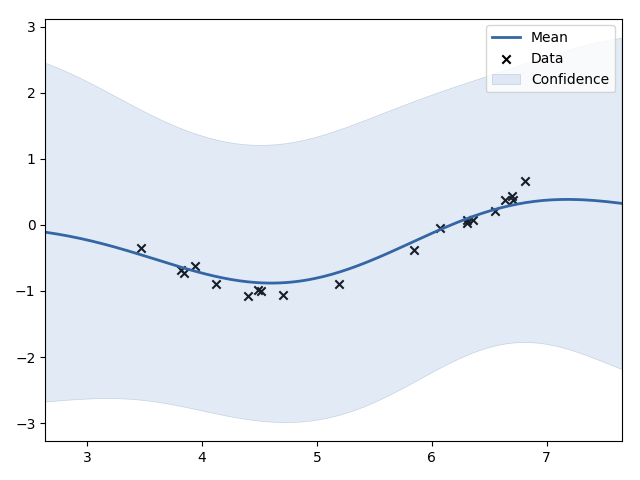
\includegraphics[scale=0.3]{example_preopt.png}
			\caption{No optimization}
		\end{subfigure}
		\begin{subfigure}[b]{0.45\linewidth}
			\centering    
			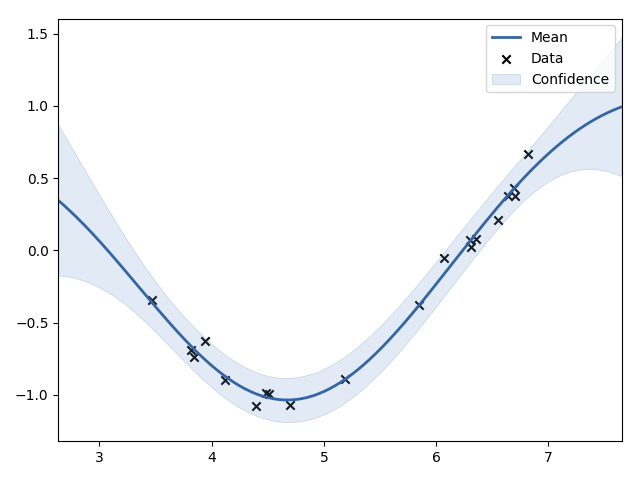
\includegraphics[scale=0.3]{example_postopt.png}
			\caption{Using \texttt{m.optimize()}}
		\end{subfigure}
		\caption{}
	\end{figure}

\end{frame}


\begin{frame}{Gaussian Process}{Bayesian Optimization}

Tuning hyperparameters for classifiers is not trivial. For smaller algorithms, gridsearch or randomsearch could for example be used. For larger models, this becomes unfeasible as the sheer time of computing an evaluation is large. Instead some policy is needed to choose the next configuration of hyperparameters to test. \linebreak 

Consider some loss-metric for the classifier as a function $f$ over the hyperparameters $X$, we would like to find the set of hyperparameters that minimizes this function. However, this function is unknown and can only be evaluated (slowly) pointwise. 

\end{frame}

\begin{frame}{Gaussian Process}{Bayesian Optimization}
The function $f$ could instead be modeled as a Gaussian process. From the GP a proposal for the optimal choice of $X$ can be generated, each new evaluation will then bring more information about the function. \linebreak

How to actually choose the proposals can be done in a multitude of ways. Since the model captures uncertainties, proposals can be put in areas of low mean, favoring \emph{Exploitation}, or in areas of high variance, favoring \emph{Exploration}. Usually an \emph{Aquisition function} is designed to balance the choice between the two extremes.
\end{frame}

\begin{frame}[fragile]{Gaussian Process}{GPyOpt}
	
Bayesian optimization tool built on top of GPy for an easy usage. \linebreak

\textbf{Example:}

Find the minimum value of the function $(6x-2)^2*\sin{12x-4}$.


\begin{Verbatim}[fontsize=\footnotesize]
def f(x):
	return (6*x - 2)**2 * np.sin(12*x-4) 

domain = [{ 'name': 'var_1', 'type': 'continuous','domain': (0, 1)}]
Bopt = BayesianOptimization(f=f, domain=domain)
Bopt.run_optimization(max_iter=5)
\end{Verbatim}


\end{frame}

\begin{frame}{Gaussian Process}{GPyOpt}


\begin{figure}[!t]
	\centering  
	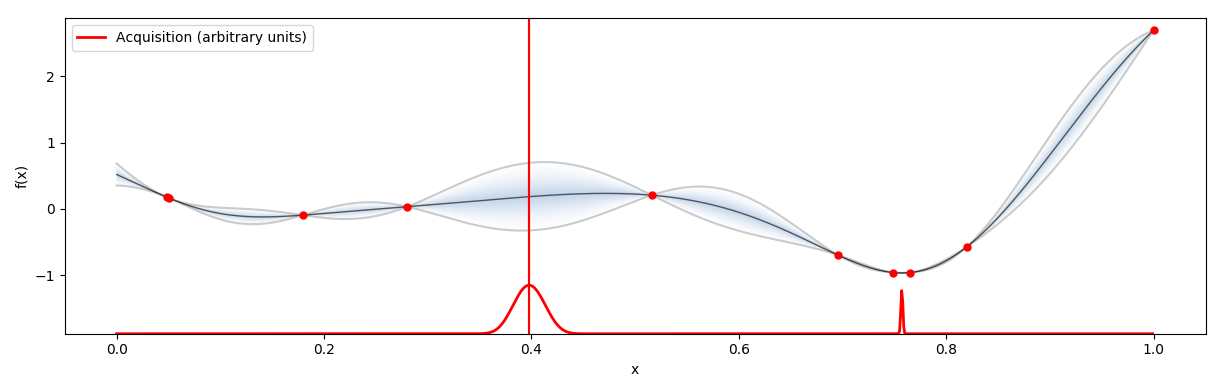
\includegraphics[scale=0.3]{bopt.png}
	\caption{The Gaussian process and acquisition function after 5 iteration steps.}
\end{figure}

\end{frame}


\bgroup
\setbeamertemplate{background}{}
\setbeamercolor{background canvas}{bg=black}
% \setbeamertemplate{navigation symbols}{}
\begin{frame}[t,plain]{}{}
  \begin{center}
    {\tiny \textcolor{white}{The End}}
  \end{center}
\end{frame}
\egroup

\end{document}
